% polyglot_optimization.tex
\begin{frame}
    \centering
    \textbf\ttfamily{\huge{A Common Interface}}
\end{frame}

\begin{frame}{Analyses and Challenges}
    \begin{figure}[h]
        \centering
        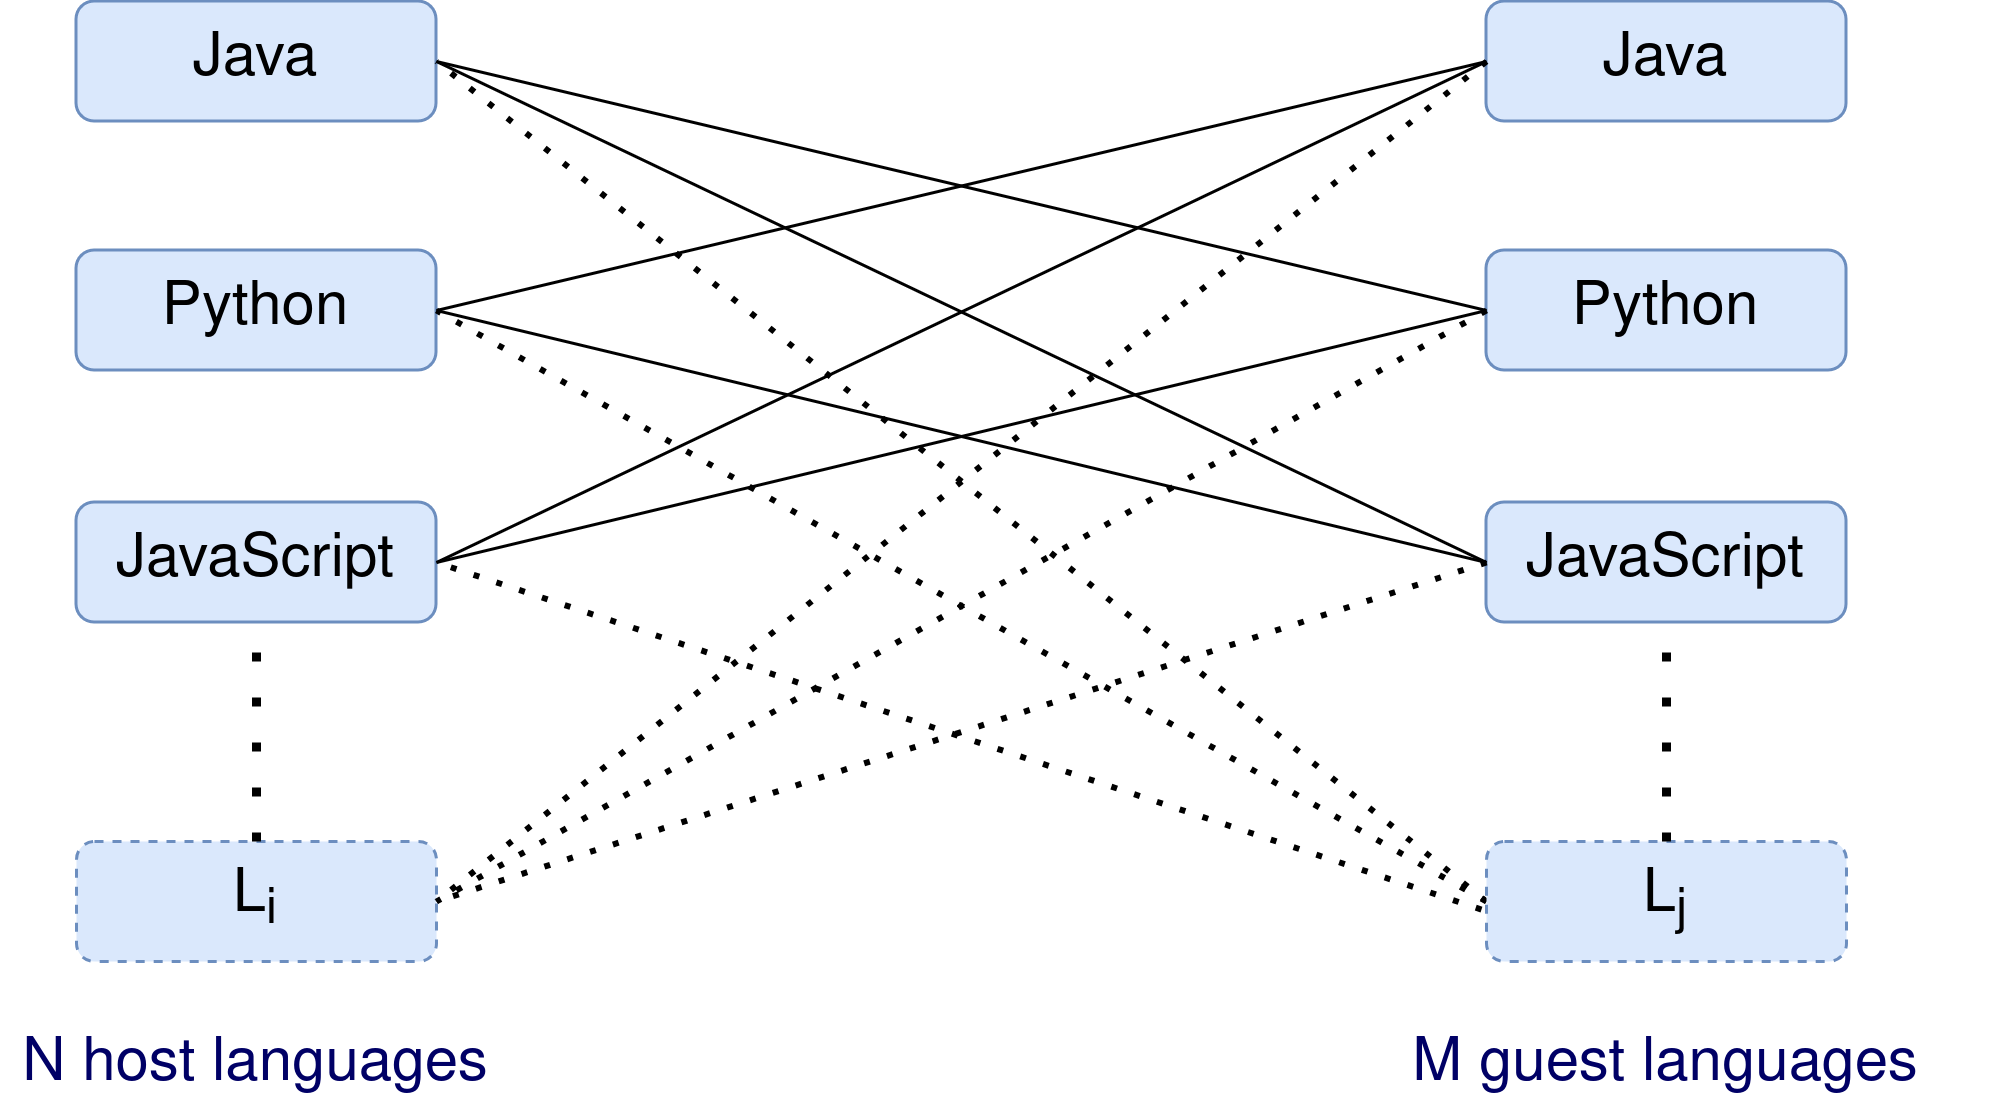
\includegraphics[width=0.6\textwidth]{images/nxm analyses}
        \caption{$NxM$ polyglot systems}
        \label{fig:figure}
    \end{figure}
    \begin{itemize}
        \item To analyze polyglot programs, one need to run interlanguage analyses.
    \end{itemize}
\end{frame}

\begin{frame}{Possible Solutions}
    \begin{itemize}
        \item Several approaches were considered for polyglot program analysis:
        \begin{enumerate}
            \vspace{3mm}
            \item Translate the guest languages to host languages.
            \vspace{3mm}
            \item Develop a new IR that can express all languages.
            \vspace{3mm}
            \item Use an existing interface that is compatible with both host and guest languages.
        \end{enumerate}
    \end{itemize}
\end{frame}


\begin{frame}[fragile]{Previous Example: Java calling Python Script}
    \begin{minipage}[b]{0.45\linewidth}
        \centering
        \begin{lstlisting}[
            frame=single,
            language=python,
            numbers=left,
            basicstyle=\tiny\ttfamily,
            caption={\normalsize{Adding complex no. in loop}},
            captionpos=b,
            backgroundcolor=\color{lightgray},   % Background color
            numberstyle=\color{pink},            % Line number color
            keywordstyle=\color{keywordcolor}\bfseries, % Keywords color
            commentstyle=\color{commentcolor},   % Comment color
            stringstyle=\color{stringcolor}      % String color
        ,label={lst:lstlisting2}]
class ComplexNumber:
def __init__(self, r, i):
    self.r = r
    self.i = i
def __add__(self, other):
    cTmp= ComplexNumber(self.r, other.i)
    return ComplexNumber(self.r+other.r+cTmp.r,
                         self.i+other.i+cTmp.i)
def __str__(self):
    return f"({self.r} + {self.i}i)"

def addComplex(i:int, n:int):
    c1 = ComplexNumber(545,n)  #python object
    c2 = ComplexNumber(9878,i) #python object
    return c1 + c2

def addComplexLoop(n: int):
    sum=0
    for i in range(10000):
        sum= sum+ addComplex(i,n).r
    return sum
        \end{lstlisting}
    \end{minipage}
    \hspace{6mm}
    \begin{minipage}[b]{0.48\linewidth}
        \centering
        \begin{lstlisting}[
            frame=single,
            language=java,
            numbers=left,
            basicstyle=\tiny\ttfamily,
            caption={Python script called from java},
            captionpos=b,
            backgroundcolor=\color{lightgray},   % Background color
            numberstyle=\color{pink},            % Line number color
            keywordstyle=\color{keywordcolor}\bfseries, % Keywords color
            commentstyle=\color{commentcolor},   % Comment color
            stringstyle=\color{stringcolor}      % String color
        ,label={lst:lstlisting2.1}]
void test() {
    String pyFile=
       "./src/main/polyglot/testCase.py";
    //create a context
    try (Context ctx = Context.create()) {
       File f= new File(pyFile);
       //load the file
       Source src= Source.
                  newBuilder("python",f).build();
       //load the py script in ctx
       ctx.eval(src);
       //getting python function
       Value pyLoop = ctx.getBindings("python")
               .getMember("addComplexLoop");
       //calling python fun
       Value result= pyLoop.execute(1000);
       System.out.println(result.asLong());
    } catch (Exception e) {
       e.printStackTrace();
    }
}
        \end{lstlisting}
    \end{minipage}
\end{frame}

\begin{frame}{Research Work}
    Our research focused on finding an existing common interface:
    \begin{itemize}
        \vspace{2mm}
        \item Experimented with Java-Python polyglot system.
        \vspace{2mm}
        \item Constructed various test programs.
        \vspace{2mm}
        \item Visually analyzed compilation graphs at different tiers of Graal and Truffle.
    \end{itemize}
\end{frame}

\begin{frame}{Tools Used}
    We used the following tools to aid us:
    \begin{itemize}
        \item \textbf{Dgraal.Dump} graal compiler flag to dump IRs from different compiler tiers
        \vspace{2mm}
        \item \textbf{Ideal Graph Visualizer(IGV)} was used to visualize the compilation dumps.
        \vspace{2mm}
        \item \textbf{Seaform} was further used to reorganise information from the dumps and remove unwanted information.
    \end{itemize}
\end{frame}
\begin{frame}{Guest Language Object Allocation}
    \begin{figure}[h]
        \centering
        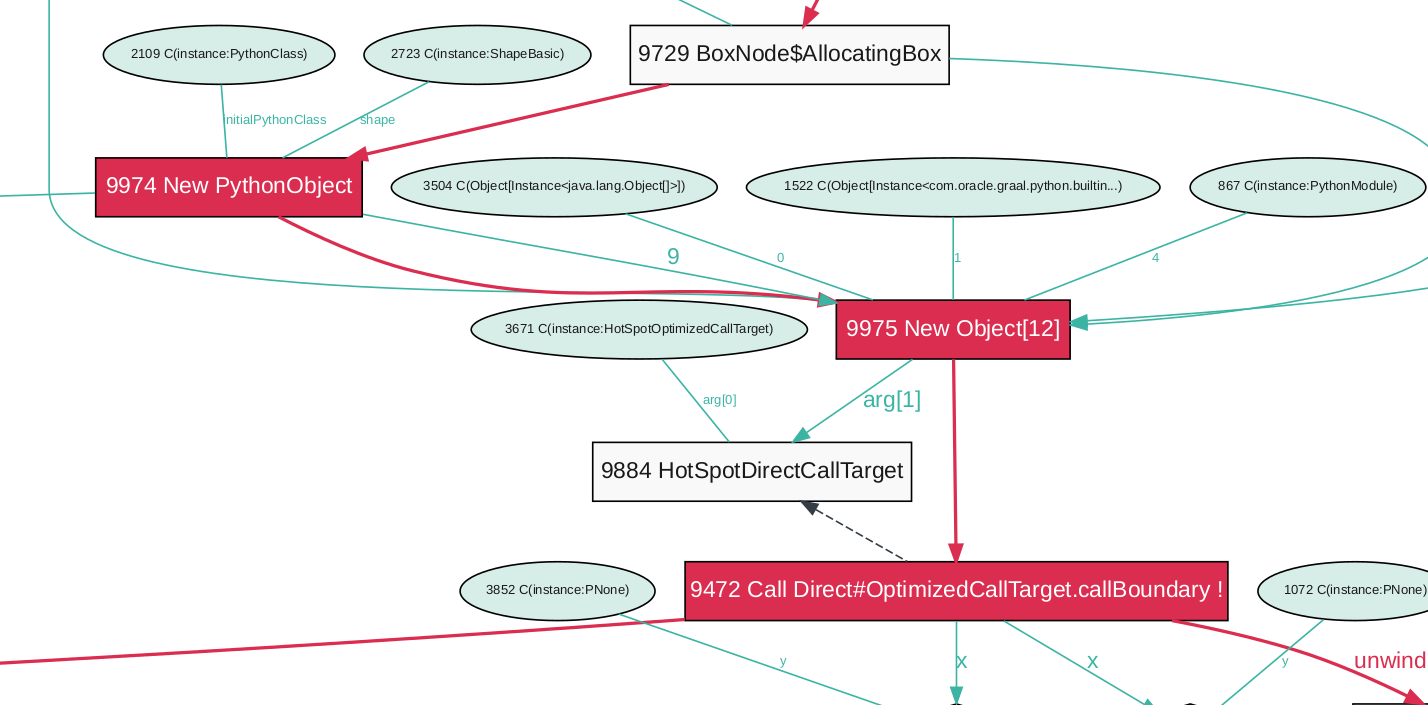
\includegraphics[width=0.8\textwidth]{images/igv_dump}
        \caption{A Python object in the output of PE}
    \end{figure}
\end{frame}
\begin{frame}{Findings}
    \begin{figure}[h]
        \centering
        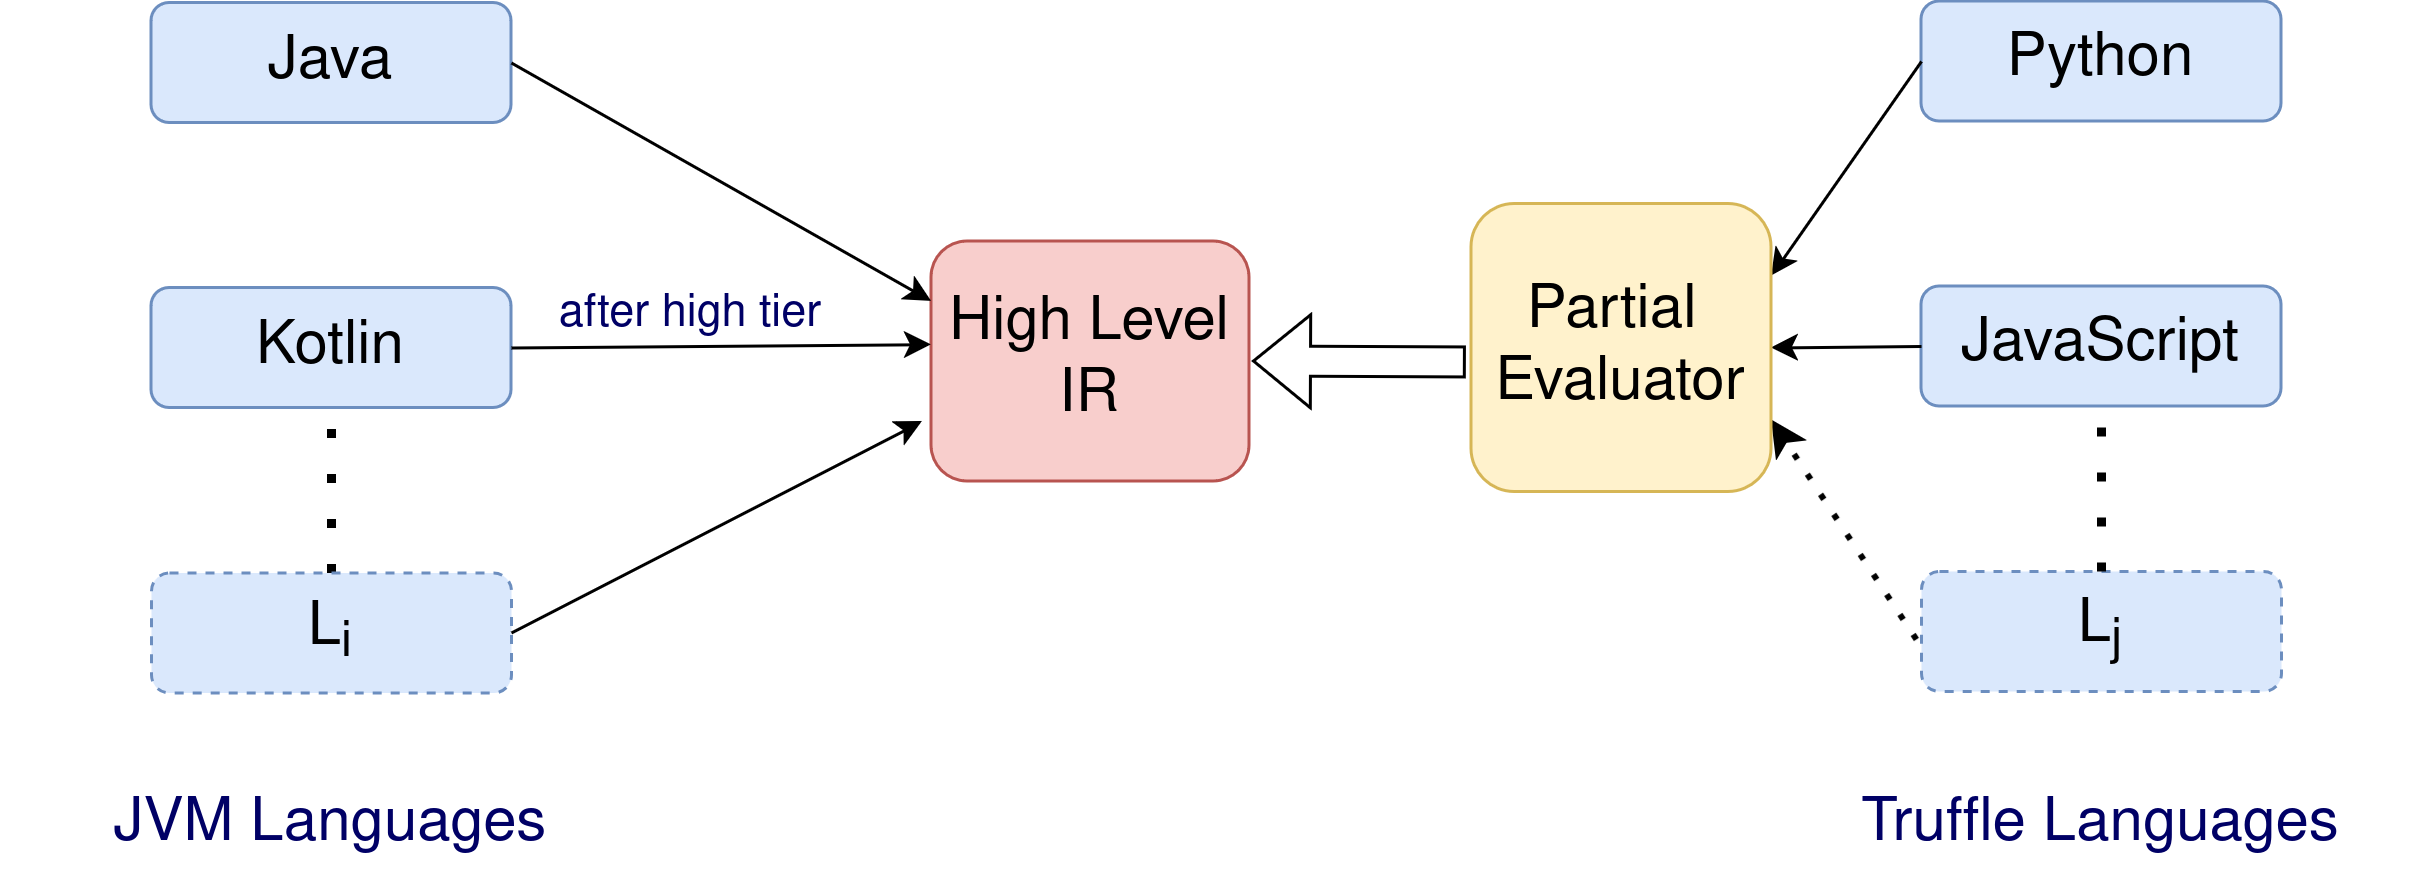
\includegraphics[width=0.6\textwidth]{images/common_interface}
        \caption{$NxM$ polyglot systems with a common interface}\label{fig:figure2}
    \end{figure}

    \begin{itemize}
        \item Truffle PE actually produces High-Level Intermediate Representation (HIR).
    \end{itemize}
\end{frame}
\begin{frame}{Proposed Solution}
    \begin{itemize}
        \item We can utilize this HIR to develop an analysis framework which will facilitate inter-procedural analyses across languages.
        \vspace{2mm}
        \item In the PYE research paper author implemented a similar framework in to make analysis more precise in OpenJDK's JIT.
        \vspace{2mm}
    \end{itemize}
\end{frame}
